% ============================================================
%  GENERATED by make_a5_test.py — do not edit; edit the generator.
%  Space — Section 1, A5 TEST of the Year 7 workbook redesign.
%  The real booklet is ../Space_Unit_Booklet_Yr7_8.tex (untouched).
%  Build: python3 make_a5_test.py && python3 fill_a5.py Space_Section1_A5
% ============================================================
\documentclass[11pt,a5paper,twoside]{article}

\usepackage{fontspec}
\setmainfont{Lato}[
  Path=../fonts/, Extension=.ttf, Ligatures=TeX,
  UprightFont=Lato-Regular, ItalicFont=Lato-Italic,
  BoldFont=Lato-Bold, BoldItalicFont=Lato-BoldItalic ]
\newfontfamily\headingfont{Poppins}[
  Path=../fonts/, Extension=.ttf, Ligatures=TeX,
  UprightFont=Poppins-Regular, ItalicFont=Poppins-Italic,
  BoldFont=Poppins-Bold, BoldItalicFont=Poppins-BoldItalic ]

% A5, mirrored: the wider margin is on the inside, by the fold.
\usepackage[a5paper, inner=17mm, outer=13mm, top=19mm, bottom=17mm,
            headheight=14pt, headsep=4mm, footskip=8mm]{geometry}
\usepackage[protrusion=true,expansion=false]{microtype}
\usepackage{xcolor}
\usepackage{tikz}
\usetikzlibrary{arrows.meta, calc, patterns}
\usepackage{tcolorbox}
\tcbuselibrary{skins, breakable}
\usepackage{fancyhdr}
\usepackage{titlesec}
\usepackage{enumitem}
\usepackage{booktabs}
\usepackage{array}
\usepackage{longtable}
\usepackage{pdflscape}
\usepackage{amsmath}
\usepackage{needspace}
\usepackage{lastpage}
\usepackage{calc}
\usepackage{graphicx}
\usepackage{ragged2e}
\usepackage[hidelinks]{hyperref}

% ── Black and white inside ──────────────────────────────────────────────────
% The body still names the master's colours; inside an A5 booklet they all
% print as ink or grey, so map them here rather than editing the text.
\definecolor{Ink}{HTML}{111111}
\colorlet{Space}{Ink}\colorlet{SpaceMid}{Ink}\colorlet{Navy}{Ink}
\colorlet{DarkGrey}{black!72}\colorlet{Grey}{black!60}\colorlet{MidGrey}{black!35}
\colorlet{Line}{black!45}\colorlet{Paper}{white}\colorlet{LightGrey}{white}
\colorlet{Gold}{Ink}\colorlet{GoldDark}{Ink}\colorlet{Teal}{Ink}\colorlet{Coral}{Ink}
\colorlet{Violet}{Ink}\colorlet{Earth}{Ink}\colorlet{EarthDark}{Ink}
\color{Ink}

% ── Page style ──────────────────────────────────────────────────────────────
\pagestyle{fancy}
\fancyhf{}
\renewcommand{\headrulewidth}{0.4pt}
\fancyhead[LE]{\headingfont\footnotesize Space}
\fancyhead[RO]{\headingfont\footnotesize\leftmark}
\fancyfoot[LE,RO]{\headingfont\footnotesize\thepage}
\fancypagestyle{opener}{\fancyhf{}\renewcommand{\headrulewidth}{0pt}%
  \fancyfoot[LE,RO]{\headingfont\footnotesize\thepage}}
\raggedbottom
\setlength{\emergencystretch}{2em}
\setlength{\parindent}{0pt}
\setlength{\parskip}{4pt plus 1pt}
\setlist{itemsep=2pt, topsep=4pt, leftmargin=1.3em}

% ── Headings ────────────────────────────────────────────────────────────────
\titleformat{\subsection}{\headingfont\large\bfseries}{\thesubsection}{0.6em}{}
\titlespacing{\subsection}{0pt}{2pt}{6pt}
\titleformat{\subsubsection}{\headingfont\normalsize\bfseries}{}{0em}{}
\titlespacing{\subsubsection}{0pt}{8pt}{2pt}
% Every lesson part starts on a new page (Kodie's booklet rule).
\let\oldsubsection\subsection
\renewcommand{\subsection}{\clearpage\oldsubsection}

% ── Lesson opener band ──────────────────────────────────────────────────────
% \lessonopener{n}{title}{ink symbol}{running head}
\newcommand{\lessonopener}[4]{%
  \clearpage\thispagestyle{opener}%
  \refstepcounter{section}\markboth{#4}{#4}%
  \noindent\begin{minipage}[b]{\dimexpr\linewidth-40mm\relax}
    {\headingfont\bfseries\footnotesize\addfontfeatures{LetterSpace=14}SPACE \textbullet\ LESSON}\par\vspace{1mm}
    {\headingfont\bfseries\fontsize{46}{44}\selectfont #1}\par\vspace{2mm}
    {\headingfont\bfseries\fontsize{15}{18}\selectfont\RaggedRight #2\par}
  \end{minipage}\hfill
  \begin{minipage}[b]{38mm}\includegraphics[width=38mm]{#3}\end{minipage}\par
  \vspace{3mm}\noindent\rule{\linewidth}{1.6pt}\par\vspace{2mm}}

% Key vocabulary: a write-in table, one row per word, rows 1.5 cm tall,
% vertical rules between columns and down both sides (Kodie's table rule).
\newcommand{\vocabrow}[1]{\rule{0pt}{5mm}\textbf{#1}\rule[-10mm]{0pt}{0pt} & \\ \hline}
\newenvironment{keyvocab}{%
  \oldsubsection*{Key vocabulary}
  {\small Write what each word means as you meet it in this lesson.}\par\smallskip
  \renewcommand{\arraystretch}{1}%
  \begin{longtable}{|>{\RaggedRight}p{30mm}|p{\dimexpr\linewidth-30mm-4\tabcolsep-3\arrayrulewidth-1pt\relax}|}
  \hline \rule{0pt}{4.2mm}\headingfont\bfseries Word & \headingfont\bfseries What it means \\[1mm] \hline \endhead}
 {\end{longtable}}

% ── Box system: told apart by frame and icon, never by colour ───────────────
% Icons in the tab: I do ● · We do ●● · You do ●●● (the gradual release,
% read as dots), Key idea ◆, Above level ▲, Country ◎.
\newcommand{\icodots}[1]{\tikz[baseline=-0.6ex]{\foreach \i in {1,...,#1}{\fill[white] (\i*1.9mm,0) circle (0.7mm);}}}
\newcommand{\icokey}{\tikz[baseline=-0.6ex]{\fill[white] (0,0.9mm)--(0.9mm,0)--(0,-0.9mm)--(-0.9mm,0)--cycle;}}
\newcommand{\icoup}{\tikz[baseline=-0.6ex]{\fill[white] (-1mm,-0.8mm)--(1mm,-0.8mm)--(0,1mm)--cycle;}}
\newcommand{\icocountry}{\tikz[baseline=-0.6ex]{\draw[white,line width=0.5pt] (0,0) circle (1mm); \fill[white] (0,0) circle (0.45mm);}}
\tcbset{wbbase/.style={enhanced, colback=white, arc=1.2mm,
    left=3mm, right=3mm, top=4mm, bottom=2.5mm, before skip=10pt, after skip=8pt,
    attach boxed title to top left={xshift=3mm, yshift=-2.4mm},
    boxed title style={colback=Ink, colframe=Ink, arc=0.8mm, boxrule=0pt,
                       left=1.6mm, right=1.8mm, top=0.6mm, bottom=0.6mm},
    fonttitle=\headingfont\bfseries\footnotesize, coltitle=white}}
\newtcolorbox{idobox}[1]{wbbase, breakable, colframe=Ink, boxrule=1pt,
  title={\icodots{1}\ I do \textbullet\ #1}}
\newtcolorbox{wedobox}[1]{wbbase, breakable, frame hidden,
  borderline={1.1pt}{0pt}{Ink, dash pattern=on 4pt off 2.6pt},
  title={\icodots{2}\ We do \textbullet\ #1}}
\newtcolorbox{youdobox}[1][Check your understanding]{wbbase, breakable=false,
  colframe=Ink, boxrule=2.4pt, top=5mm,
  title={\icodots{3}\ You do \textbullet\ #1}}
\newtcolorbox{keybox}[1]{wbbase, breakable, colframe=Ink, boxrule=0.5pt,
  title={\icokey\ #1}}
\newtcolorbox{abovebox}[1][Above level \textbullet\ Year 8 extension]{wbbase, breakable, frame hidden,
  borderline={0.6pt}{0pt}{Ink}, borderline={0.6pt}{1.6pt}{Ink},
  title={\icoup\ #1}}
\newtcolorbox{countrybox}[1]{wbbase, breakable, frame hidden,
  borderline={1.4pt}{0pt}{Ink, line cap=round, dash pattern=on 0pt off 2.4pt},
  title={\icocountry\ #1}}

% ── Questions: number on its own line, text on the next, no marks ──────────
\newcounter{qnum}[section]
\renewcommand{\theqnum}{\thesection.\arabic{qnum}}
\newcommand{\question}[2]{\refstepcounter{qnum}\par\needspace{5\baselineskip}%
  \vspace{4pt}\noindent{\headingfont\bfseries Q\theqnum}\par\nobreak
  \noindent #2\par\nobreak\vspace{2pt}}
\newcommand{\vocab}[1]{\textbf{#1}}
\newcommand{\figcap}[1]{\begin{center}\small\itshape #1\end{center}}
\newcommand{\vc}[2]{{\small\itshape VC 2.0: #1 --- #2}\par}

% ── Writing space (from the Particle Model booklet, A5 sizes) ───────────────
% Every box logs its page to \jobname.abp; fill_a5.py measures the space left
% at the foot of each page and shares it out via \jobname.abx.
\newcounter{abox}
\newwrite\abpos \immediate\openout\abpos=\jobname.abp
\newcommand{\abset}[2]{\expandafter\gdef\csname abx@#1\endcsname{#2}}
\InputIfFileExists{\jobname.abx}{}{}
\def\abgrp{0}
\newcommand{\abnext}{\stepcounter{abox}%
  \edef\abcur{\ifcsname abx@\theabox\endcsname\csname abx@\theabox\endcsname\else 0pt\fi}}
\newcommand{\ablog}{\edef\abtmp{\noexpand\write\abpos{\theabox\space\abgrp\space\noexpand\thepage}}\abtmp}
\newcommand{\abh}[1]{\dimexpr#1+\abcur\relax}
% Plain box: mathematical working.
\newcommand{\workbox}[1]{\par\abnext
  \begin{tcolorbox}[enhanced, breakable=false, arc=1.2mm, colback=white, colframe=black!45,
    left=2mm, right=2mm, top=1mm, bottom=1mm, boxrule=0.8pt, height=\abh{#1}, before skip=3pt, after skip=6pt]
  \end{tcolorbox}\ablog}
% Dotted thirds: rows 9 mm, dotted / dotted / solid, ending on a dotted line;
% the number of rows comes from the box's final height. Dots stay dark.
\newlength\thirdrow \setlength\thirdrow{9mm}
\tikzset{thirdsolid/.style={draw=black!70, line width=0.5pt},
         thirddot/.style={draw=black!70, line width=0.6pt, dash pattern=on 0.9pt off 1.6pt}}
\newlength\lbH \newlength\lbO \newcount\lbN
\newcommand{\answerbox}[1]{\par\abnext
  \setlength\lbH{\dimexpr\abh{#1}-2pt\relax}%
  \lbN=\numexpr(\dimexpr\lbH-6mm-\thirdrow/2\relax)/\thirdrow\relax
  \ifnum\lbN<1 \lbN=1 \fi
  \setlength\lbO{\dimexpr(\lbH-\lbN\thirdrow)/2\relax}%
  \begin{tcolorbox}[enhanced, breakable=false, arc=1.2mm, colback=white, colframe=black!45,
    left=2mm, right=2mm, top=1mm, bottom=1mm, boxrule=0.8pt, height=\abh{#1}, before skip=3pt, after skip=6pt,
    underlay={\begin{tcbclipinterior}
      \foreach \i in {1,...,\the\lbN}{
        \draw[thirddot] ([xshift=3mm,yshift=-\lbO-(\i-1)*\thirdrow]interior.north west) -- ([xshift=-3mm,yshift=-\lbO-(\i-1)*\thirdrow]interior.north east);
        \draw[thirddot] ([xshift=3mm,yshift=-\lbO-(\i-1)*\thirdrow-\thirdrow/3]interior.north west) -- ([xshift=-3mm,yshift=-\lbO-(\i-1)*\thirdrow-\thirdrow/3]interior.north east);
        \draw[thirdsolid] ([xshift=3mm,yshift=-\lbO-(\i-1)*\thirdrow-2*\thirdrow/3]interior.north west) -- ([xshift=-3mm,yshift=-\lbO-(\i-1)*\thirdrow-2*\thirdrow/3]interior.north east);}
      \draw[thirddot] ([xshift=3mm,yshift=-\lbO-\lbN\thirdrow]interior.north west) -- ([xshift=-3mm,yshift=-\lbO-\lbN\thirdrow]interior.north east);
    \end{tcbclipinterior}}]
  \end{tcolorbox}\ablog}

% Ink fills for the labelling diagrams (no colour inside the booklet).
\tikzset{
  ink white/.style={fill=white},
  ink light/.style={preaction={fill=white}, pattern=north east lines},
  ink mid/.style={preaction={fill=white}, pattern=crosshatch},
  ink dots/.style={preaction={fill=white}, pattern=dots},
  ink rows/.style={preaction={fill=white}, pattern=horizontal lines},
  ink solid/.style={fill=Ink}}

% ── Padding to a multiple of 4 (copier booklet mode) ────────────────────────
\newcommand{\notespage}{\clearpage\markboth{Notes}{Notes}%
  \subsection*{Notes}\vspace{2mm}%
  \begin{tikzpicture}\foreach \y in {0,...,15}{\draw[black!35, line width=0.4pt] (0,-\y*9mm) -- (\linewidth,-\y*9mm);}\end{tikzpicture}}
\newcount\padleft
\newcommand{\padtofour}{\clearpage
  \pgfmathtruncatemacro\pagesused{\the\value{page}-1}%
  \pgfmathtruncatemacro\padn{mod(4-mod(\pagesused,4),4)}%
  \padleft=\padn\relax
  \loop\ifnum\padleft>0 \notespage\advance\padleft by -1 \repeat
  \clearpage}

\begin{document}

% ---- Cover: the unit's cover art, full bleed, in colour ------------------
\thispagestyle{empty}
\begin{tikzpicture}[remember picture, overlay]
  \node at (current page.center) {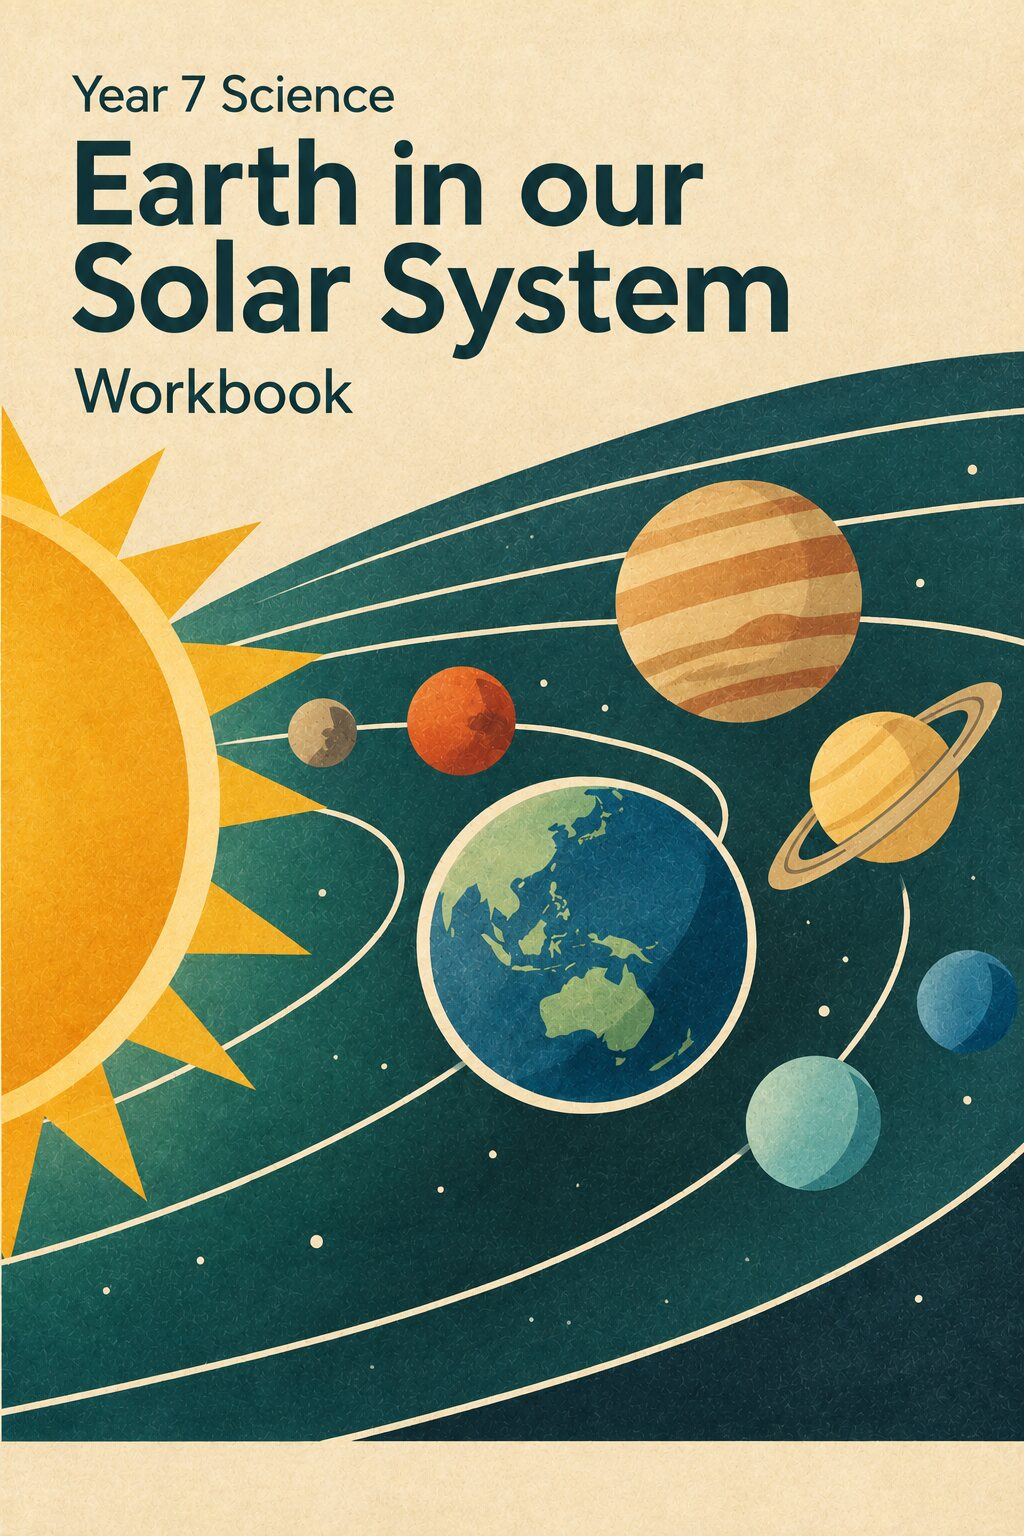
\includegraphics[width=\paperwidth, height=\paperheight, keepaspectratio=false, trim=0 40 0 40, clip]{../../../covers/earth-solar-system.jpg}};
\end{tikzpicture}
\mbox{}
\clearpage

% ---- Inside cover ---------------------------------------------------------
\thispagestyle{plain}\markboth{Space}{Space}
{\headingfont\bfseries\Large Space}\par
{\headingfont Section 1 --- A5 trial of the workbook layout}\par\vspace{5mm}
\renewcommand{\arraystretch}{2.2}
\begin{tabular}{@{}l p{78mm}@{}}
\textbf{Name} & \hrulefill \\ \textbf{Class} & \hrulefill \\ \textbf{Teacher} & \hrulefill \\
\end{tabular}
\renewcommand{\arraystretch}{1}

\begin{countrybox}{Acknowledgement of Country}
This booklet was created on the unceded Country of the Wurundjeri-Woiwurrung people of the Kulin Nation. We acknowledge Elders past, present, and emerging. Aboriginal and Torres Strait Islander peoples have read, recorded and navigated by this sky for tens of thousands of years --- the oldest continuous astronomical tradition on Earth --- and that knowledge appears throughout this unit as living science, not history.
\end{countrybox}

\begin{keybox}{How this booklet works}
Section~N goes with Lesson~N. Each kind of box has its own frame and mark:\par\smallskip
\renewcommand{\arraystretch}{1.35}
\begin{tabular}{@{}p{24mm}l@{}}
\textbf{I do} {\scriptsize\textbullet} & Your teacher works it through --- you follow \\
\textbf{We do} {\scriptsize\textbullet\textbullet} & You try it with help, together \\
\textbf{You do} {\scriptsize\textbullet\textbullet\textbullet} & On your own: check your understanding \\
\textbf{Key idea} & The idea to remember \\
\textbf{Above level} & Year 8 extension (double frame) \\
\textbf{Country} & First Nations perspectives (dotted frame) \\
\end{tabular}
\end{keybox}

% ---- Section 1 ------------------------------------------------------------
\lessonopener{1}{Earth, Moon and Sun --- Scale and Structure}{art/l1-ink.pdf}{1 \textbullet\ Earth, Moon and Sun}\label{sec:1}
\vc{Science Understanding}{Physical sciences: Earth and space sciences; scale and relative size of Earth, Moon and Sun}

\begin{keyvocab}
  \vocabrow{Empty space}
  \vocabrow{Inner core}
  \vocabrow{Outer core}
  \vocabrow{Mantle}
  \vocabrow{Crust}
  \vocabrow{Satellite}
  \vocabrow{Regolith}
  \vocabrow{Tidal locking}
  \vocabrow{Highlands}
  \vocabrow{Maria}
  \vocabrow{Main sequence star}
  \vocabrow{Nuclear fusion}
\end{keyvocab}


\subsection{The scale of Earth, Moon and Sun}\label{sub:1.1}

The three most important objects in our immediate cosmic environment differ enormously in size. Understanding their relative sizes is foundational to everything else in this unit.

\begin{center}\small
\begin{tabular}{lrrr}
\toprule
\headingfont\textbf{Object} & \headingfont\textbf{Diameter (km)} & \headingfont\textbf{Mass (kg)} & \headingfont\textbf{Distance from Earth} \\
\midrule
Moon    & 3,474          & $7.34\times10^{22}$  & 384,400 km avg \\
Earth   & 12,742         & $5.97\times10^{24}$  & ---             \\
Sun     & 1,392,000      & $1.99\times10^{30}$  & 150,000,000 km (1 AU) \\
\bottomrule
\end{tabular}
\end{center}

\begin{keybox}{Key concept: Scale}
If Earth were the size of a tennis ball (6.7 cm across), the Moon would be a marble (1.8 cm) about 1.9 m away, and the Sun would be a sphere 7.5 m across, placed 807 m down the road. The solar system is almost entirely \vocab{empty space}\label{voc:empty-space}.
\end{keybox}


\begin{youdobox}

\question{2}{Use the table to state the diameter of Earth and the diameter of the Sun.}
\answerbox{1.6cm}

\question{2}{Calculate how many times wider the Sun is than Earth. Show your working and give your answer to the nearest whole number.}
\workbox{1.6cm}

\question{2}{The Moon is 384,400 km from Earth. Calculate how many Earth diameters would fit into that gap.}
\workbox{1.6cm}

\question{2}{In the tennis-ball model, Earth is 6.7 cm across and the Sun sits 807 m down the road. Explain what this model shows that the table of diameters alone does not.}
\answerbox{1.6cm}

\end{youdobox}

\subsection{Structure of Earth}\label{sub:1.2}

Earth has four main layers:
\begin{itemize}
  \item \vocab{Inner core}\label{voc:inner-core} --- solid iron-nickel; radius \textasciitilde 1,200 km; temperature \textasciitilde 5,400°C
  \item \vocab{Outer core}\label{voc:outer-core} --- liquid iron-nickel; generates Earth's magnetic field (the dynamo effect)
  \item \vocab{Mantle}\label{voc:mantle} --- semi-solid rock; 2,900 km thick; convection currents drive plate tectonics
  \item \vocab{Crust}\label{voc:crust} --- thin, solid rock; 5--70 km thick; oceanic (denser, thinner) and continental (less dense, thicker)
\end{itemize}

\subsubsection{Diagram: Label the layers of Earth}
% Colours and band order mirror the slide-deck version of this diagram
% (deck1.html): the two outer layers in Space blue, the two core layers
% in Gold. Leader lines run out to a common rail on the right so the
% labels sit in a single column and cannot collide.
\begin{center}
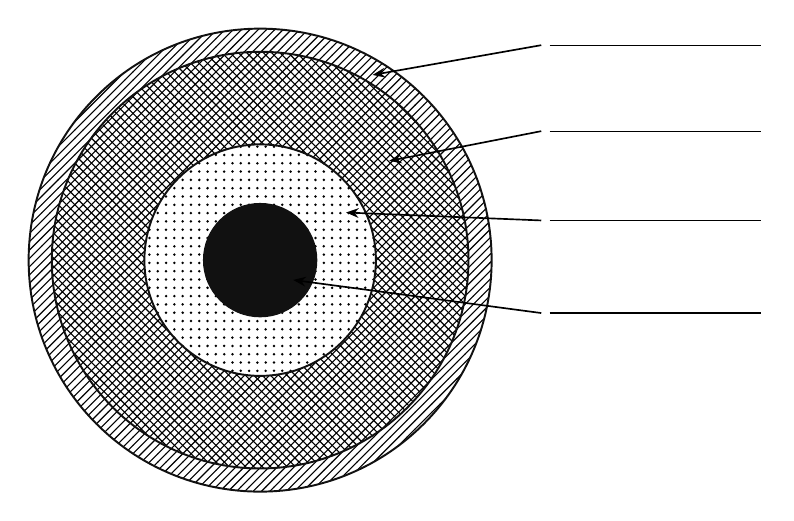
\begin{tikzpicture}[scale=0.84, every node/.style={transform shape},
    band/.style={draw=Ink, line width=0.7pt},
    lead/.style={draw=black, line width=0.6pt, -{Stealth[length=4.5pt,width=3.5pt]}},
    ansrule/.style={right, inner sep=2pt}
  ]
  \filldraw[band, ink light] (0,0) circle (3.5cm);
  \filldraw[band, ink mid] (0,0) circle (3.15cm);
  \filldraw[band, ink dots]  (0,0) circle (1.75cm);
  \filldraw[band, ink solid]  (0,0) circle (0.85cm);

  % arrowheads land inside the band being labelled
  \draw[lead] (4.25,3.25)  -- (1.70,2.8);
  \draw[lead] (4.25,1.95)  -- (1.95,1.5);
  \draw[lead] (4.25,0.60)  -- (1.30,0.72);
  \draw[lead] (4.25,-0.80) -- (0.50,-0.30);

  \node[ansrule] at (4.3,3.25)  {\rule{3.2cm}{0.5pt}};
  \node[ansrule] at (4.3,1.95)  {\rule{3.2cm}{0.5pt}};
  \node[ansrule] at (4.3,0.60)  {\rule{3.2cm}{0.5pt}};
  \node[ansrule] at (4.3,-0.80) {\rule{3.2cm}{0.5pt}};
\end{tikzpicture}

\vspace{0.6em}
{\small\textit{Word bank:}\quad Outer core \ \textbullet\ Crust \ \textbullet\ Inner core \ \textbullet\ Mantle}
\end{center}


\begin{youdobox}


\question{2}{Which layer generates Earth's magnetic field, and what is this process called?}
\answerbox{1.6cm}

\question{2}{The mantle is described as semi-solid rock. State its thickness and what its convection currents drive.}
\answerbox{1.6cm}

\question{2}{Compare oceanic and continental crust using two differences given in the booklet.}
\answerbox{1.6cm}

\end{youdobox}



\subsection{The Moon}\label{sub:1.3}

The Moon is Earth's only natural \vocab{satellite}\label{voc:satellite}. It produces no light of its own --- everything we see is reflected sunlight.

\begin{itemize}
  \item \textbf{Diameter}: 3,474 km --- about one quarter of Earth's
  \item \textbf{Distance}: 384,400 km from Earth on average; light crosses this in \textbf{1.28 seconds}
  \item \textbf{Orbital period}: 27.3 days --- and it \textit{rotates} in exactly the same time
  \item \textbf{Surface}: covered in \vocab{regolith}\label{voc:regolith}, a fine powdery rock produced by billions of years of meteorite impacts
  \item \textbf{No atmosphere} and no liquid water, so temperatures swing from $-173$\,°C at night to $+127$\,°C in daylight
\end{itemize}

\begin{keybox}{Why we only ever see one side}
The Moon's rotation period and orbital period are identical (27.3 days), so the same face is always turned towards Earth. This is called \vocab{tidal locking}\label{voc:tidal-locking}, and it is the normal outcome for a moon orbiting close to a much larger body. The hemisphere we never see from Earth is the \textbf{far side} --- not the ``dark side.'' It receives just as much sunlight as the near side.
\end{keybox}

Two kinds of terrain are visible with the naked eye. The number of craters on a surface tells you how old it is: the longer a surface has been there, the more impacts it has collected.

\begin{itemize}
  \item \vocab{Highlands}\label{voc:highlands} --- the bright, rugged regions. This is the Moon's \textbf{original crust}, so it is the oldest surface. It has been exposed to meteorite impacts for the whole history of the Moon, which is why it is so heavily cratered
  \item \vocab{Maria}\label{voc:maria} (singular \textit{mare}, Latin for ``sea'') --- the dark, flat plains. Later, huge impacts punched basins into the crust, and lava welled up and flooded them. When that lava cooled it created a \textbf{new, smooth surface}, wiping out the craters that were there before. Because this happened after the highlands formed, the maria have had less time to collect impacts --- so they are only lightly cratered
\end{itemize}


\begin{youdobox}

\question{3}{Explain why we always see the same face of the Moon from Earth.}
\answerbox{1.6cm}

\question{2}{Describe the difference between the maria and the highlands, and state which is older.}
\answerbox{1.6cm}

\question{2}{The Moon has no atmosphere. Explain how this causes its extreme temperature range.}
\answerbox{1.6cm}

\end{youdobox}



\subsection{Structure of the Sun}\label{sub:1.4}

The Sun is a \vocab{main sequence star}\label{voc:main-sequence-star} --- it converts hydrogen into helium through \vocab{nuclear fusion}\label{voc:nuclear-fusion} in its core.

\begin{itemize}
  \item \textbf{Core}: where fusion occurs; temperature \textasciitilde 15 million°C
  \item \textbf{Radiative zone}: energy moves outward as photons (takes \textasciitilde 100,000 years to cross)
  \item \textbf{Convective zone}: energy carried by convecting plasma
  \item \textbf{Photosphere}: the visible surface (\textasciitilde 5,778 K); where sunspots form
  \item \textbf{Chromosphere and Corona}: outer atmosphere; much hotter than photosphere (corona: 1--3 million K)
\end{itemize}

\subsubsection{Diagram: Label the layers of the Sun}
% Same construction as the Earth diagram in 1.2.1 — concentric bands,
% white separators, leader lines out to a common rail on the right.
% Warm palette here rather than Space blue: gold ramp for the interior,
% Coral for the fusion core and the chromosphere.
\begin{center}
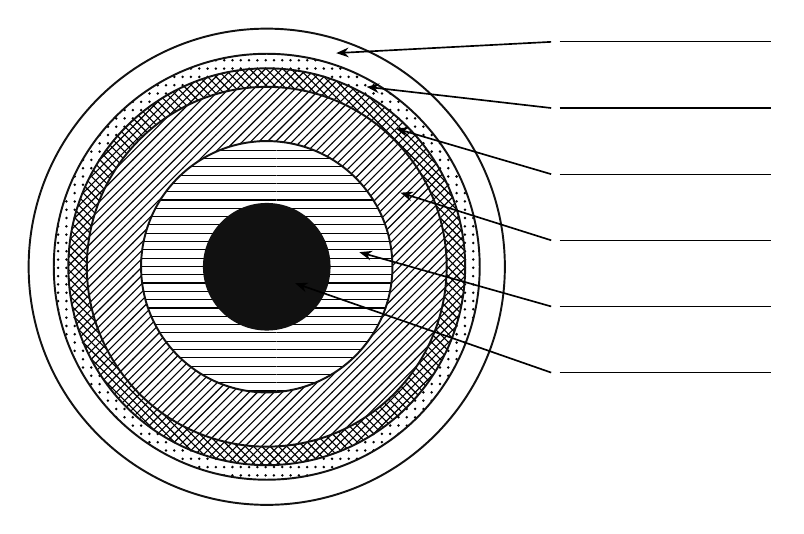
\begin{tikzpicture}[scale=0.84, every node/.style={transform shape},
    band/.style={draw=Ink, line width=0.7pt},
    lead/.style={draw=black, line width=0.6pt, -{Stealth[length=4.5pt,width=3.5pt]}},
    ansrule/.style={right, inner sep=2pt}
  ]
  \filldraw[band, ink white]     (0,0) circle (3.60cm);
  \filldraw[band, ink dots]    (0,0) circle (3.22cm);
  \filldraw[band, ink mid] (0,0) circle (3.00cm);
  \filldraw[band, ink light]     (0,0) circle (2.72cm);
  \filldraw[band, ink rows]     (0,0) circle (1.90cm);
  \filldraw[band, ink solid]    (0,0) circle (0.95cm);

  \draw[lead] (4.30,3.40)  -- (1.05,3.23);
  \draw[lead] (4.30,2.40)  -- (1.51,2.72);
  \draw[lead] (4.30,1.40)  -- (1.95,2.09);
  \draw[lead] (4.30,0.40)  -- (2.02,1.12);
  \draw[lead] (4.30,-0.60) -- (1.40,0.22);
  \draw[lead] (4.30,-1.60) -- (0.43,-0.25);

  \node[ansrule] at (4.35,3.40)  {\rule{3.2cm}{0.5pt}};
  \node[ansrule] at (4.35,2.40)  {\rule{3.2cm}{0.5pt}};
  \node[ansrule] at (4.35,1.40)  {\rule{3.2cm}{0.5pt}};
  \node[ansrule] at (4.35,0.40)  {\rule{3.2cm}{0.5pt}};
  \node[ansrule] at (4.35,-0.60) {\rule{3.2cm}{0.5pt}};
  \node[ansrule] at (4.35,-1.60) {\rule{3.2cm}{0.5pt}};
\end{tikzpicture}

\vspace{0.6em}
{\small\textit{Word bank:}\quad Convective zone \ \textbullet\ Corona \ \textbullet\ Core \ \textbullet\ Photosphere \ \textbullet\ Chromosphere \ \textbullet\ Radiative zone}
\end{center}

\begin{idobox}{Worked example: Light travel time from the Sun}
\textit{The Sun is 150,000,000 km from Earth. Light travels at 300,000 km/s. How long does sunlight take to reach us?}

\medskip
$\text{Time} = \dfrac{\text{Distance}}{\text{Speed}} = \dfrac{150{,}000{,}000 \text{ km}}{300{,}000 \text{ km/s}} = 500 \text{ s} = 8 \text{ min } 20 \text{ s}$

\medskip
\textbf{Answer}: Sunlight takes 8 minutes and 20 seconds to reach Earth. This means the Sun we see right now is actually how it looked 8 minutes ago.
\end{idobox}

\begin{wedobox}{Your turn}
A flash of light leaves the Moon. How long before we see it? (Moon is 384,400 km away; speed of light = 300,000 km/s)

\workbox{4cm}
\end{wedobox}


\begin{youdobox}

\question{2}{Define nuclear fusion as it occurs in the Sun.}
\answerbox{1.6cm}

\question{2}{State the temperature of the Sun's core and of its photosphere.}
\answerbox{1.6cm}

\question{3}{Jupiter is 5.20 AU from the Sun. Sunlight reaches Earth (1 AU) in 500 seconds. Calculate how long sunlight takes to reach Jupiter, in minutes and seconds.}
\workbox{1.6cm}

\end{youdobox}

\clearpage
\begin{abovebox}\label{y8:1.moon}
	\textbf{Year 8 Extension: How the Moon formed --- the Giant Impact Hypothesis}
	
	The leading model for the Moon's origin is the \vocab{Giant Impact Hypothesis}\label{voc:giant-impact-hypothesis}. About \textbf{4.5 billion years ago} a Mars-sized body --- named \textbf{Theia} --- struck the young Earth. The collision threw a disc of molten rock and vapour into orbit, and that material clumped together under gravity to form the Moon.
	
	\medskip
	Two pieces of evidence support it:
	\begin{itemize}
		\item The Moon has almost \textbf{no iron core}. Earth's iron had already sunk to its centre before the impact, so the debris blasted into orbit came mostly from the rocky mantle.
		\item Moon rock returned by the Apollo missions has \textbf{oxygen isotope ratios identical to Earth's}. Rock formed elsewhere in the solar system does not match --- so the Moon and Earth are made of the same material.
	\end{itemize}
	
	\medskip
	\textbf{Why it matters}: the Moon's mass stabilises Earth's axial tilt at about 23.5°. Without it, the tilt could wander between 0° and 85° over millions of years, making stable long-term climates --- and possibly complex life --- far less likely.
\end{abovebox}

\begin{abovebox}\label{y8:1.mag}
	\textbf{Year 8 Extension: Earth's magnetosphere and space weather}
	
	The liquid iron in Earth's \textbf{outer core} is constantly moving, and moving
	metal generates a magnetic field --- the \vocab{dynamo effect}\label{voc:dynamo-effect}. That field does
	not stop at the surface. It reaches tens of thousands of kilometres out into
	space, forming the \vocab{magnetosphere}\label{voc:magnetosphere}: an invisible shield around the whole
	planet.
	
	\smallskip
	It has something to shield us from.
	
	\begin{itemize}
		\item \vocab{Solar wind}\label{voc:solar-wind} --- a constant stream of charged particles blowing
		outward from the Sun at 400--800 km/s. It never stops.
		\item \vocab{Coronal mass ejections}\label{voc:coronal-mass-ejections} (CMEs) --- huge bursts of plasma thrown
		off the Sun, which can reach Earth in one to three days.
		\item \vocab{Auroras}\label{voc:auroras} --- the magnetosphere funnels charged particles toward
		the poles, where they collide with atmospheric gases and make them glow.
		This is the \textit{aurora australis} in the south and the
		\textit{aurora borealis} in the north. An aurora is what the shield
		looks like while it is working.
	\end{itemize}
	
	\smallskip
	\vocab{Space weather}\label{voc:space-weather} is the name for these events, and it has consequences on
	the ground. On 13 March 1989 a geomagnetic storm induced currents in Quebec's
	power transmission lines large enough to collapse the entire provincial grid in
	under 90 seconds, leaving about six million people without electricity for nine
	hours. Modern GPS, satellites and radio communication are all vulnerable.
	
	\medskip
	\noindent\textbf{Extension challenge.}\; Mars has no global magnetic field, and
	most of its atmosphere has been stripped away by the solar wind over billions of
	years. Earth has both a field and an atmosphere. What does the comparison suggest
	the magnetic field is doing --- and what might happen if Earth's field weakened
	a great deal?
	\workbox{5.0cm}
\end{abovebox}



% ---- Glossary, then notes pages to a multiple of 4 -------------------------
\clearpage\markboth{Glossary}{Glossary}
\subsection*{Glossary}
{\small Every key word in this section and the page it is introduced on.}\par\smallskip
\renewcommand{\arraystretch}{1.3}
\begin{longtable}{|>{\RaggedRight}p{38mm}|p{10mm}|p{\dimexpr\linewidth-48mm-6\tabcolsep-4\arrayrulewidth-1pt\relax}|}
\hline \rule{0pt}{4mm}\headingfont\bfseries Word & \headingfont\bfseries Page & \headingfont\bfseries In my own words \\ \hline \endhead
  Auroras & \pageref{voc:auroras} & \\ \hline
  Coronal mass ejections & \pageref{voc:coronal-mass-ejections} & \\ \hline
  Crust & \pageref{voc:crust} & \\ \hline
  Dynamo effect & \pageref{voc:dynamo-effect} & \\ \hline
  Empty space & \pageref{voc:empty-space} & \\ \hline
  Giant Impact Hypothesis & \pageref{voc:giant-impact-hypothesis} & \\ \hline
  Highlands & \pageref{voc:highlands} & \\ \hline
  Inner core & \pageref{voc:inner-core} & \\ \hline
  Magnetosphere & \pageref{voc:magnetosphere} & \\ \hline
  Main sequence star & \pageref{voc:main-sequence-star} & \\ \hline
  Mantle & \pageref{voc:mantle} & \\ \hline
  Maria & \pageref{voc:maria} & \\ \hline
  Nuclear fusion & \pageref{voc:nuclear-fusion} & \\ \hline
  Outer core & \pageref{voc:outer-core} & \\ \hline
  Regolith & \pageref{voc:regolith} & \\ \hline
  Satellite & \pageref{voc:satellite} & \\ \hline
  Solar wind & \pageref{voc:solar-wind} & \\ \hline
  Space weather & \pageref{voc:space-weather} & \\ \hline
  Tidal locking & \pageref{voc:tidal-locking} & \\ \hline
\end{longtable}
\padtofour
\end{document}
